\section{Filter}
\writtenby{\dcauthornameriren}%
Für viele Bildverarbeitungsprozesse werden Filter genutzt, die sich z.B. der mathematischen Faltung bedienen, um Rauschen zu entfernen, Kanten zu schärfen oder auch Kanten zu erkennen.
Die zur Bildverbesserung benutzen Filter, werden hier kurz erläutert.

\subsection*{Pixelbasierte Bildverbesserung}
Bei der pixelbasierten Bildverbesserung wird jeder Pixelfarbwert einzeln berechnet, ohne auf die Umgebung dieses Pixels Rücksicht zu nehmen.
Die so neu entstandenen Werte ersetzen die alten Farbwerte des Pixels.
So kann das Bild z.B. aufgehellt und der Kontrast verstärkt werden.
\begin{figure}[H]
  \centering
  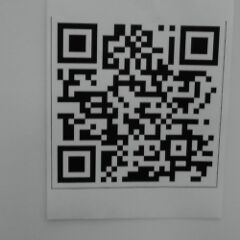
\includegraphics[height=4cm]{img/QR/perfect_real_01.jpg}
  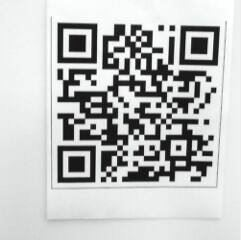
\includegraphics[height=4cm]{img/QR/qr-bright.jpg}
  \caption{Pixelbasierte Bildverbesserung.}
  \label{fig:pixelbright}
\end{figure}
%Quelle Tönnies2005

\subsection*{Faltungsfilter}
Faltungsfilter, auch lineare Filter genannt, machen sich das Prinzip der Faltung zu Nutzen, das bereits im Abschnitt der "`Kantenerkennung"' beschrieben ist.

Im Fall der Bildbearbeitung gibt es weitere Anwendungsmöglichkeiten für ent\-sprechende Faltungsmatrizen, z.B. für die Schärfung des Bildes oder der Ausgleich von Rauschen.
Für den Rauschausgleich gibt es eine Spezialform dieser Faltungsfilter, die \surname{Gauß}-Filter genannt wird, und bei der die Faltungsmatrix den Werten einer \surname{Gauß}-Glocke, mit dem Maximum in der Mitte der Matrix, entspricht.
Dadurch erreicht man eine ausgleichende Wirkung auf verrauschte Bilder, denn alle Pixel werden an ihre umgebenden Pixel angepasst, was aber zusätzlich den Effekt hat, dass das Bild unschärfer wird.

\begin{equation}
  K_{sharpen} = \begin{vmatrix}
    -1 & -1 & -1 \\
    -1 &  9 & -1 \\
    -1 & -1 & -1
  \end{vmatrix}
  \quad
  K_{Gauss} = \begin{vmatrix}
    \frac{1}{16} & \frac{1}{8} & \frac{1}{16} \\
    \frac{1}{ 8} & \frac{1}{4} & \frac{1}{ 8} \\
    \frac{1}{16} & \frac{1}{8} & \frac{1}{16}
  \end{vmatrix}
\end{equation}
\begin{figure}[H]
  \centering
  
\includegraphics[height=4cm]{img/QR/perfect_03.jpg}
  
\includegraphics[height=4cm]{img/QR/qr-gauss.jpg}
  
\includegraphics[height=4cm]{img/QR/qr-sharp.jpg}
  \caption[Beispiel \surname{Gauss}-Filter]{Original, Anwendung von \surname{Gauss}-Filter und anschließender Schärfefilterung}
  \label{fig:sharpgauss}
\end{figure}
%Quelle Tönnies2005

\subsection*{Unscharfes Maskieren}
\label{sec:unsharp}
%sharpenimage
Beim unscharfen Maskieren, wird ein Originalbild verdreifacht und eine Version davon, mit z.B. einem \surname{Gauß}-Filter, unscharf gemacht.
Danach wird dieses unscharfe Bild von der zweiten Version abgezogen, insofern ein Schwellwert überschritten ist, und so ein Bild mit hervorgehobenen Kanten erhalten.
Dieses wird zum dritten Bild addiert und in diesem dadurch die Kanten verstärkt, was einer Schärfung des Originalbildes entspricht.
\begin{figure}[H]
  \centering
  
\includegraphics[height=4cm]{img/QR/blurry_03_3.jpg}
  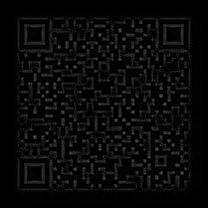
\includegraphics[height=4cm]{img/QR/qr-unsharpmask.jpg}
  
\includegraphics[height=4cm]{img/QR/qr-unsharpmask-sharp.jpg}
  \caption[unscharfes Maskieren mit \surname{Gauß}-Filter]{unscharfes Maskieren mit \surname{Gauß}-Filter (Original, Maske, Ergebnis)}
  \label{fig:unsharpmask}
\end{figure}


\subsection*{\surname{Laplace}-Operator}
%isBlurry
Den Verlauf von Kanten kann man auch durch die zweite Ableitung über den Pixelwerten des Bildes erhalten.
Denn dort wo diese von positiven zu negativen Werten wechselt, besitzt die erste Ableitung ein Maximum und somit an dieser Stelle einen sehr starken Helligkeitsunterschied im Bild, welcher auf eine Kante hindeutet.
Dieser Vorzeichenwechsel wird auch als Nulldurchgang bezeichnet.
Der \surname{Laplace}-Operator berechnet sich mit
\begin{equation}
  \nabla^2 f(x,y) = \frac{\partial^2 f}{\partial x^2}(x,y) + \frac{\partial^2 f}{\partial y^2}(x,y) + \frac{\partial^2 f}{\partial x \partial y}(x,y) + \frac{\partial^2 f}{\partial y \partial x}(x,y)
\end{equation}
Für eine schnellere Berechnung können aber auch 2 angenäherte Faltungsmatrizen genutzt werden.
\begin{equation}
  K_4 = \begin{vmatrix}
     0 & -1 &  0 \\
    -1 &  4 & -1 \\
     0 & -1 &  0
  \end{vmatrix}
  \quad
  K_8 = \begin{vmatrix}
    -1 & -1 & -1 \\
    -1 &  8 & -1 \\
    -1 & -1 & -1
  \end{vmatrix}
\end{equation}
\begin{figure}[H]
  \centering
  
\includegraphics[height=4cm]{img/QR/perfect_03.jpg}
  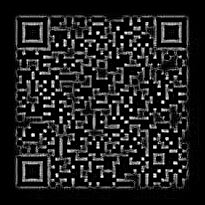
\includegraphics[height=4cm]{img/QR/qr-laplace.jpg}
  \caption[Beispiel \surname{Laplace}-Filter]{Original mit \surname{Laplace}-Filter~($K_8$)}
  \label{fig:laplace}
\end{figure}
%Quelle Tönnies2005 S 182



\subsection*{Laplacian-of-Gaussian-Filter}
\label{sec:LoG}
%isBlurry
Der \surname{Laplace}-Operator allein ist durch die Reaktion auf jeden stärkeren Helligkeitsunterschied sehr empfindlich für Rauschen und wird deswegen auch zusammen mit einem \surname{Gauß}-Filter verwendet.
Durch diese Kombination wird das Rauschen abgeschwächt, aber die Reaktivität auf Kanten bleibt erhalten. Dieser Filter wird auch \surname{Marr}-\surname{Hildreth}-Filter oder auch Mexican-Hat-Filter~(wegen des Aussehens des Filters) genannt. Für die Berechnung werden die zweiten Ableitungen der \surname{Gauß}-Funktion benötigt:
\begin{equation}
  LoG(x,y) = -\frac{1}{\pi \sigma^4}(1-\frac{x^2 + y^2}{2\sigma^2}) exp(-\frac{x^2 + y^2}{2\sigma^2})
\end{equation}
Diesen Filter kann man sich noch auf andere Weise zu nutzen machen, denn die positiven Werte des \surname{Laplace}-Operators repräsentieren, wie stark die erste Ableitung ansteigt und damit wie stark die Veränderungen von Pixelpaar zu Pixelpaar ist. Somit ergibt sich daraus ein Wert für die Unschärfe des Bildes, der maximale Wert im aktuellen Bild beschreibt diese zum Beispiel. Um so größer er ist, um so schärfer ist das Bild und wenn er kleiner ist, ist auch das Bild unschärfer.
\begin{figure}[H]
  \centering
  
\includegraphics[height=4cm]{img/QR/perfect_03.jpg}
  
\includegraphics[height=4cm]{img/QR/qr-LoG.jpg}
  \caption[Beispiel Laplacian-of-Gaussian-FIlter]{Original mit Laplacian-of-Gaussian-Filter}
  \label{fig:LoG}
\end{figure}
%Quelle Tönnies2005 S 183

